%!TEX root=../document.tex

\section{Ergebnisse}
\label{sec:Ergebnisse}

Zu finden ist mein Beispiel auf Github unter \url{https://github.com/tfellner-tgm/SYT-rmi} \cite{repo}

\subsection{CORBA}

CORBA erm\"oglicht einem, Objekte \"uber mehrere Prozesse und sogar durch das Netzwerk verwendbar zu machen. Im Gegensatz zu RMI ist dies aber Programmiersprachen unabh\"angig, doch das Prinzip ist sehr \"ahnlich.

In dieser Graphik ist Erk\"ahrung wie das ganze funktioniert
\begin{figure}[!h]
        \begin{center}
                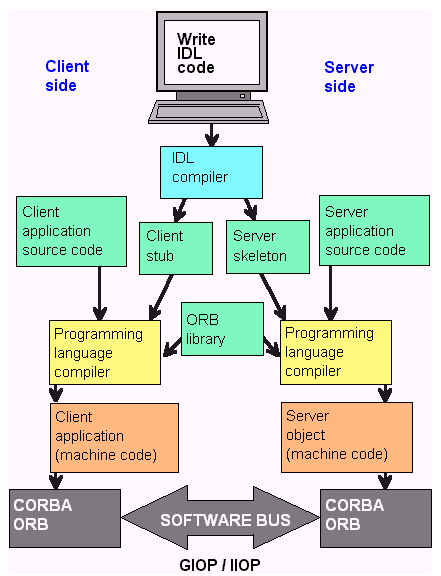
\includegraphics[width=0.5\linewidth]{images/corba_design.png}
                \caption{CORBA Erk\"ahrung \url{"http://www.pcmag.com/encyclopedia/term/40365/corba"}}
        \end{center}
\end{figure}

\clearpage

\subsection{Konfiguration und Installation}

Hier ist erkl\"art wie man die 2 ORBs, JacORB f\"ur Java und OmniORB f\"ur C++ bzw. auch Python, aufsetzt.
\\
Zuerst m\"ussen die binaries von OmniORB und JacORB mittels z.B. \texttt{wget} installiert werden. 

\begin{lstlisting}[style=bash, caption=Download von OmniORB und JacORB]
wget https://sourceforge.net/projects/omniorb/files/omniORB/omniORB-4.2.1/omniORB-4.2.1-2.tar.bz2/download
wget http://www.jacorb.org/releases/3.7/jacorb-3.7-binary.zip
\end{lstlisting}

Um OmniORB zu installieren muss man ein build directory erstellen im Ordner des extrahierten tars. \\
Danach wird \texttt{../configure} ausgef\"urt in diesem build Ordner, um die n\"otigen \texttt{make} dateien zu generieren. \\
Um \texttt{make} ausf\"uhren zu k\"onnen, m\"ussen die Packages \texttt{build-essential}, f\"ur gcc, make ... und \texttt{libpython2.7-dev}, f\"ur Python, installiert werden.\\
Danach kann der \texttt{make} Befehl angewandt werden und um es dann noch zu installieren \texttt{make install}\\
Da Libraries hinzugef\"ugt wurden, muss die \texttt{LD\_LIBRARY\_PATH} Variable noch geupdated werden mittels \texttt{ldconfig} \\
Da ich mit den OmniORB Namingservice arbeite muss dieser vor einem Test gestartet werden. Um ihn starten zu k\"onnen muss aber noch der Ordner \texttt{/var/omninames} erstellt werden.
Nun kann der Service mittels \texttt{omniNames -start -always} gestartet werden.\\

F\"ur JacORB muss zuerst die \texttt{openjdk-8-jdk} installiert werden. Da wir binaries installiert haben kann man den ungezipten Folder in \texttt{~/opt/} geben und dort dann ein Symlink zu der aktuellsten Version machen.\\

Zur Testung beider ORBS habe ich das halloWelt Beispiel \cite{halloWelt-bsp} verwendet. Wobei hier die directories richtig gesetzt werden m\"ussen (von mike zu dem Homeverzeichnis des Users) und dann der Client mittels \texttt{ant run-client} und der Server mittels \texttt{make run} gestartet werden.

\clearpage

\subsection{Programm}

Ich habe das Hallo Welt Beispiel \cite{halloWelt-bsp} zu einem simplen Rechner umge\"andert. 

Im Vergleich zu RMI ist das \texttt{UnicastRemoteObject} hier das \texttt{orb} (Object Request Broker) Objekt, diese k\"ummert sich um den Austausch der Objekte. POA (Portable Object Adapter) leitet die Aufrufe weiter an die Konkrete Implementierung, damit die orb vom tat\"achlichen Code getrennt sind.

\begin{lstlisting}[language=C++, caption=server.cc main Klasse welches die ORB und POA Objekte erstellt]
int main(int argc, char **argv)
{
  try {
    CORBA::ORB_var orb = CORBA::ORB_init(argc, argv);
    
    CORBA::Object_var obj = orb->resolve_initial_references("RootPOA");
    PortableServer::POA_var poa = PortableServer::POA::_narrow(obj);

    Calculation* calc = new Calculation();

    PortableServer::ObjectId_var calcid = poa->activate_object(calc);
    
    // Obtain a reference to the object, and register it in
    // the naming service.
    obj = calc->_this();

    CORBA::String_var x;
    x = orb->object_to_string(obj);
    cout << x << endl;

    if( !bindObjectToName(orb, obj) )
      return 1;

    calc->_remove_ref();
    
    PortableServer::POAManager_var pman = poa->the_POAManager();
    pman->activate();
    
    orb->run();
  }
  catch(CORBA::SystemException& ex) {
    cerr << "Caught CORBA::" << ex._name() << endl;
  }
  catch(CORBA::Exception& ex) {
    cerr << "Caught CORBA::Exception: " << ex._name() << endl;
  }
  catch(omniORB::fatalException& fe) {
    cerr << "Caught omniORB::fatalException:" << endl;
    cerr << "  file: " << fe.file() << endl;
    cerr << "  line: " << fe.line() << endl;
    cerr << "  mesg: " << fe.errmsg() << endl;
  }
  return 0;
}
\end{lstlisting}

\clearpage

Hier ist dann zu sehen wie ein Objekt gebindet wird.
\begin{lstlisting}[language=C++, caption=server.cc main Klasse welches die ORB und POA Objekte erstellt]
static CORBA::Boolean
bindObjectToName(CORBA::ORB_ptr orb, CORBA::Object_ptr objref)
{
  CosNaming::NamingContext_var rootContext;
  // Obtain a reference to the root context of the Name service:
  CORBA::Object_var obj;
  obj = orb->resolve_initial_references("NameService");

  // Narrow the reference returned.
  rootContext = CosNaming::NamingContext::_narrow(obj);

  try {
    // Bind a context called "test" to the root context:
    CosNaming::Name contextName;
    contextName.length(1);
    contextName[0].id   = (const char*) "test";       // string copied
    contextName[0].kind = (const char*) "my_context"; // string copied

    CosNaming::NamingContext_var testContext;
    try {
      // Bind the context to root.
      testContext = rootContext->bind_new_context(contextName);
    }
    catch(CosNaming::NamingContext::AlreadyBound& ex) {
      CORBA::Object_var obj;
      obj = rootContext->resolve(contextName);
      testContext = CosNaming::NamingContext::_narrow(obj);
    }

    // Bind objref with name Calculate to the testContext:
    CosNaming::Name objectName;
    objectName.length(1);
    objectName[0].id   = (const char*) "Calculation";   // string copied
    objectName[0].kind = (const char*) "Object"; // string copied

    try {
      testContext->bind(objectName, objref);
    }
    catch(CosNaming::NamingContext::AlreadyBound& ex) {
      testContext->rebind(objectName, objref);
    }
  }
  catch(CORBA::TRANSIENT& ex) {
    cerr << "Caught system exception TRANSIENT -- unable to contact the "
         << "naming service." << endl
         << "Make sure the naming server is running and that omniORB is "
         << "configured correctly." << endl;

    return 0;
  }
  catch(CORBA::SystemException& ex) {
    cerr << "Caught a CORBA::" << ex._name()
         << " while using the naming service." << endl;
    return 0;
  }
  return 1;
}

\end{lstlisting}

\clearpage

Das IDL File wird verwendet um die Interfaces zu generieren, welche dann von Java und C++ verwendet werden.

\begin{lstlisting}[language={[CORBA]IDL}, caption=calculator.idl Interface]
#ifndef __CALCULATOR_IDL__
#define __CALCULATOR_IDL__
module calculator {
	exception DivisionThroughZero {
		string message;
	};

	interface Calculation {
		double add(in double nr1, in double nr2);
		double subtract(in double nr1, in double nr2);
		double multiply(in double nr1, in double nr2);
		double divide(in double nr1, in double nr2) raises (DivisionThroughZero);
	};
};
#endif  // __CALCULATOR_IDL__


\end{lstlisting}

Wie vorhin erw\"ahnt braucht das Programm noch Konkrete Implementierungen dieses Interfaces.

\begin{lstlisting}[language=C++, caption=C++ IDL Implementation]
class Calculation : public POA_calculator::Calculation
{
public:
    inline Calculation() {}
    virtual ~Calculation() {}
    virtual double add(const double nr1, const double nr2);
    virtual double subtract(const double nr1, const double nr2);
    virtual double multiply(const double nr1, const double nr2);
    virtual double divide(const double nr1, const double nr2);
};


double Calculation::divide(const double nr1, const double nr2) {
    if(nr2 == 0) {
        throw calculator::DivisionThroughZero("Division by zero is undefined");
    }

    return CORBA::Double (nr1 / nr2);
}

double Calculation::add(const double nr1, const double nr2) {
    return CORBA::Double (nr1 + nr2);
}

double Calculation::subtract(const double nr1, const double nr2) {
    return CORBA::Double (nr1 - nr2);
}

double Calculation::multiply(const double nr1, const double nr2) {
    return CORBA::Double (nr1 * nr2);
}
\end{lstlisting}

\clearpage

Diese Methoden k\"onnen dann von Java mittels dem hier erzeugtem Objekt ...

\begin{lstlisting}[style=java, caption=Client.java JacORB Verbindung]
public static Calcultion connectToRemote(String[] args) {
	try {
		/* Erstellen und intialisieren des ORB */
		ORB orb = ORB.init(args, null);

		/* Erhalten des RootContext des angegebenen Namingservices */
		Object o = orb.resolve_initial_references("NameService");

		/* Verwenden von NamingContextExt */
		NamingContextExt rootContext = NamingContextExtHelper.narrow(o);

		/* Angeben des Pfades zum Calculate Objekt */
		NameComponent[] name = new NameComponent[2];
		name[0] = new NameComponent("test","my_context");
		name[1] = new NameComponent("Calculation", "Object");

		/* Aufloesen der Objektreferenzen  */
		return CalculationHelper.narrow(rootContext.resolve(name));

	} catch (Exception e) {
		System.err.println("Es ist ein Fehler aufgetreten: " + e.getMessage());
		e.printStackTrace();

		return null;
	}
}

\end{lstlisting}

... aufgerufen werden.

\begin{lstlisting}[style=java, caption=Client.java JacORB Verbindung]
public static void main(String[] args)  {

	//create Calculator Object
	Calculation calculator = connectToRemote(args);
	System.out.println("5 + 2 = " + calculator.add(5, 2));
	System.out.println("2 - 3 = " + calculator.subtract(2, 3));
	System.out.println("2 * 4.35 = " + calculator.multiply(2, 4.35));

	try {
		System.out.println("5.2 / 2.5 = " + calculator.divide(5.2, 2.5));

		//Exception Erzeugen
		calculator.divide(1,0);
	}catch(DivisionThroughZero e) {
		System.err.println(e.message);
	}
}
\end{lstlisting}

\clearpage

\section{Zeitaufzeichnung}

\renewcommand{\arraystretch}{1.5}
\begin{table}[!h]
	\center
	\begin{tabular}{ | {\hspace{3mm}} | {\hspace{3mm}} | {\hspace{3mm}} | {\hspace{3mm}} | }
		\hline \textbf{Datum} & \textbf{Erwartete Dauer} & \textbf{Reale Dauer} & \textbf{Beschreibung}\\ \hline\hline
		            29.4.2016 & 4 Stunden                & 4 Stunden            & Tutorial zum Laufen bringen fertigstellen\\ \hline
                    4.5.2016 & 2 Stunden                 & 3 1/2 Stunden        & Hallo Welt umschreiben \\ \hline
		            5.5.2016 & 3 Stunde                  & 2 Stunde             & Protokoll beginnen\\ \hline
		            5.5.2016 & 2 Stunden                 & 3 Stunden            & Fertigstellung\\ \hline
		            6.5.2016 & 2 Stunden                 & 3 Stunden            & Protokoll ferigstellen \\ \hline
	\end{tabular}
	\caption{Zeitaufzeichnung}
	\label{methoden}
\end{table}